% Unnumbered front-matter chapter. The historical portrait is an unmodified
% photograph; all surrounding graphic elements are original TikZ artwork.
\begingroup
\thispagestyle{empty}
\phantomsection
\addcontentsline{toc}{chapter}{人物介绍：庞特里亚金}
\hypersetup{allcolors=covergray}
\begin{tikzpicture}[remember picture,overlay]
\begin{scope}[shift={(current page.south west)},x=1mm,y=1mm,
  line cap=butt,line join=miter,
  every node/.style={inner sep=0pt,outer sep=0pt,text=coverink}]
  \clip (0,0) rectangle (210,297);
  \fill[coverpaper] (0,0) rectangle (210,297);
  \fill[coverred] (0,0) rectangle (6,297);

  \node[anchor=west,font=\sffamily\fontsize{10}{12}\selectfont]
    at (18,282) {人物介绍 · 谨向原作者致敬};
  \node[anchor=east,font=\coverru\fontsize{8}{10}\selectfont]
    at (192,282) {ПАМЯТИ МАТЕМАТИКА};
  \draw[coverink,line width=0.65pt] (18,276) -- (192,276);
  \node[anchor=north west,font=\sffamily\bfseries\fontsize{32}{36}\selectfont]
    at (17,271) {庞特里亚金};
  \node[anchor=west,font=\sffamily\fontsize{12}{15}\selectfont]
    at (18,247) {列夫·谢苗诺维奇·庞特里亚金};
  \node[anchor=west,font=\coverru\bfseries\fontsize{14}{17}\selectfont]
    at (18,237) {Лев Семёнович Понтрягин};

  \draw[coverred,line width=2.4pt] (145,245) -- (198,276);
  \fill[coverink] (153,249) rectangle (192,271);
  \node[text=coverpaper,font=\coverru\bfseries\fontsize{23}{26}\selectfont]
    at (172.5,263) {1908};
  \node[text=coverpaper,font=\coverru\bfseries\fontsize{23}{26}\selectfont]
    at (172.5,254) {1988};

  % Keep the entire historical photograph, including hands and writing desk.
  \fill[coverred] (22,146) rectangle (112,218);
  \node[anchor=north west] at (18,222)
    {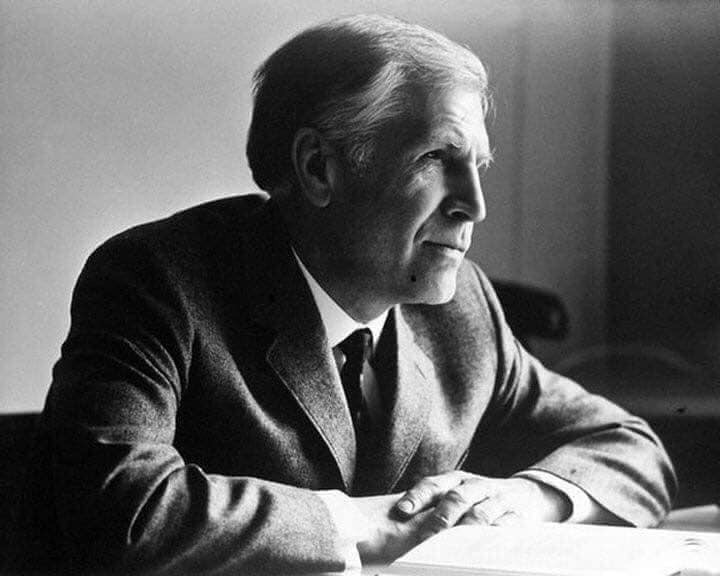
\includegraphics[width=90mm]{assets/portraits/pontryagin-c1950.jpg}};
  \draw[coverink,line width=0.6pt] (18,150) rectangle (108,222);
  \node[anchor=north west,text width=91mm,align=left,
    font=\sffamily\fontsize{7.1}{10}\selectfont,text=covergray]
    at (18,142) {约 1950 年，摄影者不详。原图等比缩放。\\
    莫斯科大学历史博物馆 / \href{https://commons.wikimedia.org/wiki/File:Понтрягин_Лев_Семёнович.jpg}{Wikimedia Commons}\\
    \href{https://creativecommons.org/licenses/by/4.0/}{CC BY 4.0}；照片来源、署名与许可见链接。};

  \node[anchor=north west,font=\sffamily\bfseries\fontsize{15}{18}\selectfont]
    at (120,222) {从拓扑到控制};
  \fill[coverred] (120,210) rectangle (137,212);
  \node[anchor=north west,text width=72mm,align=left,
    font=\sffamily\fontsize{10.1}{15}\selectfont]
    at (120,205) {庞特里亚金是苏联数学家，生于莫斯科。他早年的工作横跨代数与拓扑；庞特里亚金对偶性、特征类等成果，成为现代数学的重要\mbox{组成部分。\textsuperscript{[1]}}\\[1.2mm]
    少年时，他因意外失明。母亲塔季扬娜长期为他朗读科学文献、记录公式、整理手稿，支持他继续学习与研究。她的劳动，也是这段数学史的一部分。\textsuperscript{[2]}};

  \draw[coverink,line width=0.65pt] (18,126) -- (192,126);
  \node[anchor=west,font=\sffamily\bfseries\fontsize{12}{15}\selectfont]
    at (18,119) {生平与工作};
  \node[anchor=west,font=\coverru\fontsize{7}{9}\selectfont,text=covergray]
    at (18,111) {ЖИЗНЬ И ТРУДЫ};

  % A compact chronology. Dates and affiliations follow the institutional
  % biography, not an inferred timeline based on publication translations.
  \draw[coverred,line width=1pt] (20,104) -- (20,52);
  \foreach \yy/\yr/\txt in {
    104/1929/{莫斯科大学毕业},
    91/1934/{进入斯捷克洛夫研究所},
    78/{1950s}/{转向微分方程与最优控制},
    65/1961/{四人合著最优过程专著},
    52/1970/{创办莫大最优控制教研室}}{
    \fill[coverred] (20,\yy) circle[radius=1.25mm];
    \node[anchor=north west,font=\coverru\bfseries\fontsize{9.5}{11}\selectfont]
      at (25,\yy+2) {\yr};
    \node[anchor=north west,font=\sffamily\fontsize{7.8}{10}\selectfont]
      at (25,\yy-3.5) {\txt};
  }

  % Constructivist study: a saddle phase portrait carried by an oblique beam.
  % The concentric frame and parallel rails echo the cover's engineering lines.
  % All trajectories satisfy xy = C for x' = x, y' = -y.
  \node[anchor=west,font=\coverru\bfseries\fontsize{9}{11}\selectfont]
    at (102,120) {СЕДЛО};
  \node[anchor=east,text=covergray,font=\sffamily\fontsize{7}{9}\selectfont]
    at (190,120) {相平面 · 鞍点};
  \draw[coverink,line width=0.55pt] (102,116.5) -- (124,116.5);
  \fill[coverred] (102,116) rectangle (109,117);

  % A shared local frame keeps the beam, rails and end tick exactly aligned.
  \begin{scope}[shift={(147,88)},rotate=-28]
    \fill[coverred] (-48,-4.5) rectangle (48,4.5);
    \draw[coverink,line width=0.65pt] (-43,6.5) -- (48,6.5);
    \draw[covergray,line width=0.45pt] (-48,-6.5) -- (48,-6.5);
    \draw[coverink,line width=0.65pt] (48,4.7) -- (48,8.3);
  \end{scope}

  % Both diamonds share (147,88); corresponding sides are exactly parallel.
  \draw[coverink,line width=0.65pt]
    (147,117) -- (176,88) -- (147,59) -- (118,88) -- cycle;
  \draw[coverred,line width=1.1pt] (118,88) -- (147,59);
  \draw[covergray,line width=0.45pt] (105,88) -- (189,88);
  \draw[covergray,line width=0.45pt] (147,59) -- (147,117);
  \fill[coverink] (104,87) rectangle (106,89);
  \fill[coverred] (146.1,116.1) rectangle (147.9,117.9);

  % Preserve the black diamond and the four white hyperbola families.
  \fill[coverink] (147,113.5) -- (172.5,88) -- (147,62.5) -- (121.5,88) -- cycle;
  \begin{scope}[shift={(147,88)},scale=1.1087]
    \clip (0,23) -- (23,0) -- (0,-23) -- (-23,0) -- cycle;
    \foreach \g in {-18,-12,...,18}{
      \draw[coverpaper!12!coverink,line width=0.3pt] (\g,-23) -- (\g,23);
      \draw[coverpaper!12!coverink,line width=0.3pt] (-23,\g) -- (23,\g);
    }
    \foreach \c in {12,36,72}{
      \draw[coverpaper!92!coverink,line width=0.8pt]
        plot[domain=0.5:23,samples=90,smooth,variable=\t]
          (\t,{\c/\t})
        plot[domain=23:0.5,samples=90,smooth,variable=\t]
          ({-\t},{-\c/\t})
        plot[domain=0.5:23,samples=90,smooth,variable=\t]
          (\t,{-\c/\t})
        plot[domain=23:0.5,samples=90,smooth,variable=\t]
          ({-\t},{\c/\t});
    }
    \draw[coverpaper!75!coverink,line width=0.55pt] (-21,0) -- (21,0);
    \draw[coverpaper!75!coverink,line width=0.55pt] (0,-21) -- (0,21);
    % Separate paths give all four separatrices their own time-direction arrow.
    \foreach \sgn in {-1,1}{
      \draw[coverred,line width=1.25pt,-{Stealth[length=1.8mm]}]
        ({\sgn*9},0) -- ({\sgn*19},0);
      \draw[coverred,line width=1.25pt,-{Stealth[length=1.8mm]}]
        (0,{\sgn*19}) -- (0,{\sgn*9});
    }
    \fill[coverpaper] (-0.65,-0.65) rectangle (0.65,0.65);
  \end{scope}

  % Sparse external labels keep the mathematical object legible at book scale.
  \node[anchor=west,font=\fontsize{8}{10}\selectfont]
    at (182,91) {$x$};
  \node[anchor=west,font=\fontsize{8}{10}\selectfont]
    at (151,115) {$y$};
  \node[rotate=90,anchor=west,text=covergray,
    font=\coverru\fontsize{6.5}{8}\selectfont]
    at (193,84) {ФАЗОВЫЙ ПОРТРЕТ};
  \fill[coverink] (115,50.5) rectangle (178,57.5);
  \fill[coverred] (110,50.5) rectangle (113,57.5);
  \node[text=coverpaper,font=\fontsize{9}{11}\selectfont]
    at (146.5,54) {$\dot x=x\qquad\dot y=-y\qquad xy=C$};
  \draw[coverink,line width=0.6pt] (181,52) -- (190,52) (181,54) -- (187,54);

  \fill[coverred] (18,35) -- (192,35) -- (192,44) -- (43,44) -- (18,39) -- cycle;
  \node[text=coverpaper,anchor=west,font=\sffamily\fontsize{10}{12}\selectfont]
    at (25,39) {向他的数学创造致敬，也向他的同行、他的家人与他的师友致意。};

  \node[anchor=north west,text width=174mm,align=left,text=covergray,
    font=\sffamily\fontsize{7}{9.5}\selectfont]
    at (18,29) {\textbf{资料依据}\quad
      [1] \href{https://cs.msu.ru/persons/47}{莫斯科大学：人物档案（cs.msu.ru/persons/47）}；
      [2] \href{https://mathshistory.st-andrews.ac.uk/Biographies/Pontryagin/}{O'Connor 与 Robertson：MacTutor 传记}。\\[0pt]
      [3] \href{https://search.rsl.ru/ru/record/01006401476}{俄罗斯国立图书馆：1961 年俄文初版书目（四位作者署名）}。
      生卒日期：1908.09.03 / 1988.05.03。\\
      资料查阅：2026 年 10 月 21 日。传记为据上述资料编写的中文摘要；“编者致意”为本项目原创文字。};
\end{scope}
\end{tikzpicture}
\null\clearpage
\endgroup
